% Chapter 5: Theoretical Analysis
\section{理论对比分析}

\subsection{数据划分方式对比}

\subsubsection{划分空间与边界形状}

三种索引在数据划分方式上有本质区别,如表\ref{tab:partition-compare-detail}所示。

\begin{table}[htbp]
    \centering
    \caption{数据划分方式详细对比}
    \label{tab:partition-compare-detail}
    \begin{tabular}{lccc}
        \toprule
        \textbf{Aspect} & \textbf{MVP Tree} & \textbf{CGH Tree} & \textbf{LP Tree} \\
        \midrule
        Partition Space & Metric Space & Metric Space & Pivot Space \\
        Partition Method & Nested Spheres & Hyperplanes & Linear Hyperplanes \\
        Boundary Shape & Concentric Spheres & Distance Difference & Orthogonal Planes \\
        Number of Children & $2^k = 8$ & $2^{k-1} = 4$ & $2^k = 8$ \\
        Balance Guarantee & Median-based & Sign-based & Median-based \\
        \bottomrule
    \end{tabular}
\end{table}

\textbf{MVP树}:采用嵌套球形划分,每个pivot独立将数据分为内球和外球两部分。边界是以pivot为圆心的同心球面。

\textbf{CGH树}:采用超平面组合划分,基于距离差的符号进行划分。边界是由$\delta_{12}=0$和$\delta_{13}=0$定义的两个超平面。

\textbf{线性划分树}:在支撑点空间中采用正交划分,边界是与坐标轴垂直的超平面。

\subsubsection{划分平衡性分析}

\textbf{MVP树和LP树}:使用中位数进行划分,理论上保证每层划分的平衡性。但由于嵌套划分,后续层可能出现不平衡。

\textbf{CGH树}:基于距离差符号划分,平衡性依赖于数据分布。在某些分布下可能严重不平衡。

图\ref{fig:balance-analysis}展示了不同划分策略的平衡性特点。

\begin{figure}[htbp]
    \centering
    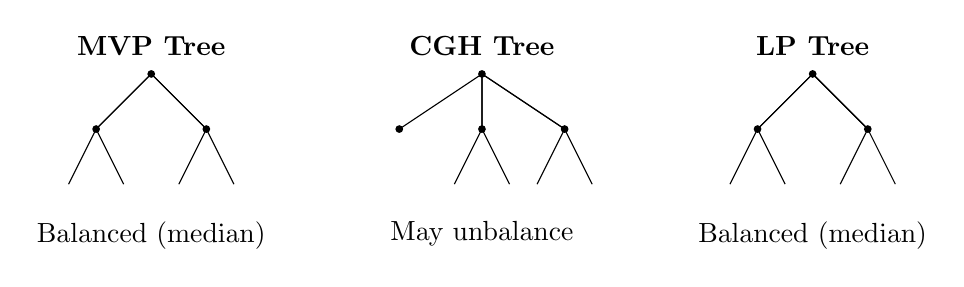
\begin{tikzpicture}[scale=0.7]
        % MVP Tree balance
        \begin{scope}[xshift=0cm]
            \node at (2,3.5) {\textbf{MVP Tree}};
            \draw (2,3) -- (1,2) -- (0.5,1);
            \draw (2,3) -- (1,2) -- (1.5,1);
            \draw (2,3) -- (3,2) -- (2.5,1);
            \draw (2,3) -- (3,2) -- (3.5,1);
            \fill (2,3) circle (2pt);
            \fill (1,2) circle (2pt);
            \fill (3,2) circle (2pt);
            \node[below] at (2,0.5) {Balanced (median)};
        \end{scope}
        
        % CGH Tree (potentially unbalanced)
        \begin{scope}[xshift=6cm]
            \node at (2,3.5) {\textbf{CGH Tree}};
            \draw (2,3) -- (0.5,2);
            \draw (2,3) -- (2,2) -- (1.5,1);
            \draw (2,3) -- (2,2) -- (2.5,1);
            \draw (2,3) -- (3.5,2) -- (3,1);
            \draw (2,3) -- (3.5,2) -- (4,1);
            \fill (2,3) circle (2pt);
            \fill (0.5,2) circle (2pt);
            \fill (2,2) circle (2pt);
            \fill (3.5,2) circle (2pt);
            \node[below] at (2,0.5) {May unbalance};
        \end{scope}
        
        % LP Tree balance
        \begin{scope}[xshift=12cm]
            \node at (2,3.5) {\textbf{LP Tree}};
            \draw (2,3) -- (1,2) -- (0.5,1);
            \draw (2,3) -- (1,2) -- (1.5,1);
            \draw (2,3) -- (3,2) -- (2.5,1);
            \draw (2,3) -- (3,2) -- (3.5,1);
            \fill (2,3) circle (2pt);
            \fill (1,2) circle (2pt);
            \fill (3,2) circle (2pt);
            \node[below] at (2,0.5) {Balanced (median)};
        \end{scope}
    \end{tikzpicture}
    \caption{三种索引的划分平衡性示意}
    \label{fig:balance-analysis}
\end{figure}

\subsection{支撑点使用效率对比}

\subsubsection{距离信息利用方式}

三种索引利用pivot距离信息的方式不同:

\begin{itemize}
    \item \textbf{MVP树}:独立使用每个pivot的距离值$d(x, p_i)$
    \item \textbf{CGH树}:使用pivot对的距离差$\delta_{ij} = d(x, p_i) - d(x, p_j)$
    \item \textbf{LP树}:联合使用距离向量$(d_1, d_2, d_3)$
\end{itemize}

\subsubsection{信息利用效率分析}

\textbf{MVP树}:每个pivot独立贡献剪枝信息,信息利用相对独立。剪枝条件是对各维度分别检查。

\textbf{CGH树}:利用pivot对之间的距离差,这包含了更多的相对位置信息。但只有$k-1$个独立的距离差变量。

\textbf{LP树}:在支撑点空间中统一利用所有距离信息,但映射过程可能导致信息损失(距离扭曲)。

\subsection{剪枝能力分析}

\subsubsection{剪枝条件对比}

表\ref{tab:pruning-compare}对比了三种索引的剪枝条件。

\begin{table}[htbp]
    \centering
    \caption{剪枝条件对比}
    \label{tab:pruning-compare}
    \begin{tabular}{ll}
        \toprule
        \textbf{Index} & \textbf{Pruning Condition} \\
        \midrule
        MVP Tree & $\exists j: d_j + r < L_{i,j}$ or $d_j - r > U_{i,j}$ \\
        CGH Tree & $\delta_{jk}^q - 2r > U_{jk}^i$ or $\delta_{jk}^q + 2r < L_{jk}^i$ \\
        LP Tree & $\exists j: d_j^q + r < L_i^j$ or $d_j^q - r > U_i^j$ \\
        \bottomrule
    \end{tabular}
\end{table}

\subsubsection{剪枝效果影响因素}

\textbf{数据分布}:
\begin{itemize}
    \item 聚类分布:MVP树和LP树效果较好,球形/立方体边界更有效
    \item 均匀分布:CGH树可能更有效,超平面划分更均匀
\end{itemize}

\textbf{查询半径}:
\begin{itemize}
    \item 小半径:所有索引效果都好
    \item 大半径:剪枝效果普遍下降,CGH树下降更快
\end{itemize}

\textbf{数据维度}:
\begin{itemize}
    \item 低维:所有索引效果都好
    \item 高维:受维度灾难影响,剪枝效果下降
\end{itemize}

\subsubsection{包含规则分析}

\textbf{MVP树}具有包含规则:若$d_j + U_{i,j} \leq r$,则子树$i$中所有数据都是查询结果,可以批量返回。

\textbf{CGH树}没有直接的包含规则,需要记录额外信息才能实现。

\textbf{LP树}有近似包含规则:在支撑点空间中判断,但不等于度量空间中的包含。

\subsection{时空复杂度分析}

\subsubsection{构建复杂度}

设数据量为$n$,pivot数为$k$(本实验$k=3$)。

\begin{table}[htbp]
    \centering
    \caption{构建复杂度分析}
    \label{tab:build-complexity}
    \begin{tabular}{lccc}
        \toprule
        \textbf{Operation} & \textbf{MVP Tree} & \textbf{CGH Tree} & \textbf{LP Tree} \\
        \midrule
        Pivot Selection (FFT) & $O(n \cdot k)$ & $O(n \cdot k)$ & $O(n \cdot k)$ \\
        Distance Computation & $O(n \cdot k)$ & $O(n \cdot k)$ & $O(n \cdot k)$ \\
        Partition & $O(n)$ & $O(n)$ & $O(n)$ \\
        Total per Level & $O(n \cdot k)$ & $O(n \cdot k)$ & $O(n \cdot k)$ \\
        Total (balanced) & $O(n \cdot k \cdot \log n)$ & $O(n \cdot k \cdot \log n)$ & $O(n \cdot k \cdot \log n)$ \\
        \bottomrule
    \end{tabular}
\end{table}

\subsubsection{查询复杂度}

\textbf{最好情况}:根节点剪枝,$O(k)$距离计算。

\textbf{最坏情况}:遍历所有节点,$O(n)$距离计算。

\textbf{平均情况}:依赖于剪枝率,通常为$O(k \cdot \log n + m)$,其中$m$为结果数量。

\subsubsection{空间复杂度}

\begin{table}[htbp]
    \centering
    \caption{空间复杂度分析}
    \label{tab:space-complexity}
    \begin{tabular}{lcc}
        \toprule
        \textbf{Index} & \textbf{Per Node} & \textbf{Total} \\
        \midrule
        MVP Tree & $O(k + 2^k \cdot k)$ & $O(n)$ \\
        CGH Tree & $O(k + 2^{k-1} \cdot 2)$ & $O(n)$ \\
        LP Tree & $O(k + 2^k \cdot k)$ & $O(n)$ \\
        \bottomrule
    \end{tabular}
\end{table}

\subsection{优缺点总结}

\subsubsection{MVP树优缺点}

\textbf{优点}:
\begin{itemize}
    \item 球形划分直观,易于理解和实现
    \item 具有包含规则,可批量返回结果
    \item 中位数划分保证平衡性
    \item 扩展自VP树,理论基础成熟
\end{itemize}

\textbf{缺点}:
\begin{itemize}
    \item 嵌套划分可能导致子区域形状复杂
    \item pivot之间的信息没有联合利用
    \item 8个子树可能有空子树
\end{itemize}

\textbf{适用场景}:低维聚类数据,需要批量返回结果的场景。

\subsubsection{CGH树优缺点}

\textbf{优点}:
\begin{itemize}
    \item 充分利用pivot对之间的距离差信息
    \item 剪枝规则与GH树一脉相承
    \item 4个子区域,树更紧凑
\end{itemize}

\textbf{缺点}:
\begin{itemize}
    \item 没有包含规则
    \item 划分平衡性依赖数据分布
    \item 距离差信息的利用不够直观
\end{itemize}

\textbf{适用场景}:数据分布较均匀,查询半径较小的场景。

\subsubsection{线性划分树优缺点}

\textbf{优点}:
\begin{itemize}
    \item 在支撑点空间中划分,可利用多维索引理论
    \item 线性边界简洁,计算效率高
    \item 剪枝条件清晰直观
\end{itemize}

\textbf{缺点}:
\begin{itemize}
    \item 支撑点空间距离是度量空间距离的下界,可能保守
    \item 距离扭曲可能影响划分质量
    \item 包含判断不精确
\end{itemize}

\textbf{适用场景}:数据在支撑点空间中分布较好的场景。
